\documentclass{beamer}
\usepackage[utf8]{inputenc}

\usetheme{Madrid}
\usecolortheme{default}
\usepackage{amsmath,amssymb,amsfonts,amsthm}
\usepackage{txfonts}
\usepackage{tkz-euclide}
\usepackage{listings}
\usepackage{adjustbox}
\usepackage{array}
\usepackage{tabularx}
\usepackage{gvv}
\usepackage{lmodern}
\usepackage{circuitikz}
\usepackage{tikz}
\usepackage{graphicx}

\setbeamertemplate{page number in head/foot}[totalframenumber]

\usepackage{tcolorbox}
\tcbuselibrary{minted,breakable,xparse,skins}



\definecolor{bg}{gray}{0.95}
\DeclareTCBListing{mintedbox}{O{}m!O{}}{%
  breakable=true,
  listing engine=minted,
  listing only,
  minted language=#2,
  minted style=default,
  minted options={%
    linenos,
    gobble=0,
    breaklines=true,
    breakafter=,,
    fontsize=\small,
    numbersep=8pt,
    #1},
  boxsep=0pt,
  left skip=0pt,
  right skip=0pt,
  left=25pt,
  right=0pt,
  top=3pt,
  bottom=3pt,
  arc=5pt,
  leftrule=0pt,
  rightrule=0pt,
  bottomrule=2pt,
  toprule=2pt,
  colback=bg,
  colframe=orange!70,
  enhanced,
  overlay={%
    \begin{tcbclipinterior}
    \fill[orange!20!white] (frame.south west) rectangle ([xshift=20pt]frame.north west);
    \end{tcbclipinterior}},
  #3,
}
\lstset{
    language=C,
    basicstyle=\ttfamily\small,
    keywordstyle=\color{blue},
    stringstyle=\color{orange},
    commentstyle=\color{green!60!black},
    numbers=left,
    numberstyle=\tiny\color{gray},
    breaklines=true,
    showstringspaces=false,
}
%------------------------------------------------------------
%This block of code defines the information to appear in the
%Title page
\title %optional
{9-9.5-1}
\date{November 6, 2024}
%\subtitle{A short story}

\author % (optional)
{Harsha Vardhan Reddy - EE24BTECH11063}



\begin{document}


\frame{\titlepage}
\begin{frame}{Question}
Find the area of the region\\
\begin{align*}
    \cbrak{\brak{x,y}:x^2+y^2\le 16a^2\;\text{and}\;y^2\le6ax}
\end{align*}

\end{frame}
\begin{frame}{allowframebreaks}
\frametitle{Curves}

    \centering
    
    \label{tab:parameters}
	\begin{tabular}[12pt]{ |c| c|}
    \hline
    \textbf{Curves}\\ 
    \hline
     $x^2+y^2\le16a^2$ \\
    \hline 
     $y^2\le6ax$\\
    \hline
    \end{tabular}
\end{frame}


\begin{frame}{Parameters Table}
    \begin{table}[ht]
    \begin{adjustbox}{width=0.8\framewidth}
       \begin{tabular}{|c|c|c|}
    \hline
     Parameter & Description & Value \\
    \hline
     $R$ & Resistance & ?\\
     \hline
     $C$ & Capacitance  & ?\\
     \hline
      $R_1$ & Resistance & 1000\\
    \hline
    $\omega_{dB}$ & Cut-off frequency & 1000\\ 
   \hline
    $A_V$ & Gain Transfer & $\dfrac{ V_{out}}{V_{in}}$ \\
    \hline
\end{tabular}
    \end{adjustbox}
    \vspace{0.5cm}
    \caption{Parameters}
    \label{tab:Gate.ee.54.1}
\end{table}
\end{frame}
\begin{frame}{allowframebreaks}
\frametitle{Inputs}

    \centering
    
    \label{tab:parameters}
	\begin{tabular}[12pt]{ |c| c|}
    \hline
    \textbf{Conic}& \textbf{Parameters}\\ 
    \hline
     $V_1$& $\myvec{0 & 0 \\ 0 & 1}$\\
    \hline 
     $u_1$& $\myvec{-3a\\0}$\\
    \hline
     $f_1$& $0$\\
     \hline
     $V_2$& $\myvec{1 & 0 \\ 0 & 1}$\\
    \hline 
     $u_2$& $\myvec{0\\0}$\\
    \hline
     $f_2$& $-16a^2$\\
     \hline
    \end{tabular}
\end{frame}
\begin{frame}
\frametitle{Solution}
The equation of a parabola in Matrix form is
\begin{align}
\vec{x}^\top\vec{V_1}\vec{x} + 2\vec{u_1}^\top\vec{x} + f_1 = 0
\end{align}
The equation of a circle in Matrix form is
\begin{align}
\vec{x}^\top\vec{V_2}\vec{x} + 2\vec{u_2}^\top\vec{x} + f_2 = 0
\end{align}

For the given parabola $y^2=6ax$, The values of $\vec{V_1}$,$\vec{u_1}$,$f_1$ are
\begin{align}
\vec{V_1}&=\myvec{0 & 0\\0 & 1}\\
\vec{u_1}&=\myvec{-3a\\0}\\
f_1&=0
\end{align}
\end{frame}
\begin{frame}
\frametitle{Solution}
For the given circle $x^2+y^2=16a^2$, The values of $\vec{V_2}$,$\vec{u_2}$,$f_2$ are
\begin{align}
\vec{V_2}&=\myvec{1 & 0\\0 & 1}\\
\vec{u_2}&=\myvec{0\\0}\\
f_2&=-16a^2
\end{align}
The intersection of two conics with parameters $V_i,u_i,f_i,\;i= 1,2$ is defined as
\begin{align}
x^T\brak{V_1+\mu V_2}x+2\brak{u_1+\mu u_2}^T x + \brak{f_1+\mu f_2}\;=\;0
\end{align}
Solving this the points of intersection are
\begin{align}
\myvec{2a\\\sqrt{12}a}\;,\;\myvec{2a\\-\sqrt{12}a}
\end{align}
\end{frame}
\begin{frame}
\frametitle{Solution}
Area between the curves is,
\begin{align}
2\int_{0}^{\sqrt{12}a} \brak{\sqrt{16a^2-y^2}-\frac{y^2}{6a}} \, dy \\
=\frac{16\pi+4\sqrt{3}a^2}{3}
\end{align}

\end{frame}
\begin{frame}{Enclosed Area Between Parabola and Circle for \( a = 1.0 \)}
    \begin{center}
        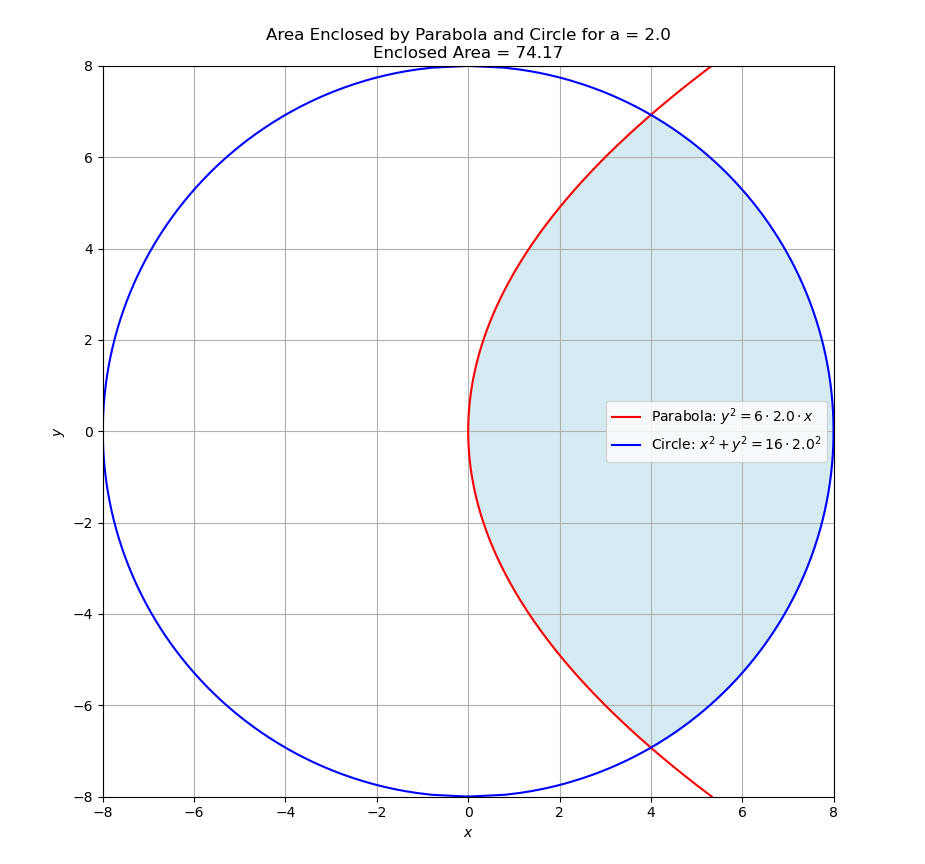
\includegraphics[width=0.7\textwidth]{figs/fig_2.png}
    \end{center}
    \vspace{0.5cm}
    \begin{itemize}
        \item The plot shows the intersection and enclosed area between the parabola \( y^2 = 6 \cdot 1.0 \cdot x \) (red) and the circle \( x^2 + y^2 = 16 \cdot 1.0^2 \) (blue).
        \item Calculated enclosed area: 18.54.
    \end{itemize}
\end{frame}
\begin{frame}{Enclosed Area Between Parabola and Circle for \( a = 2.0 \)}
    \begin{center}
        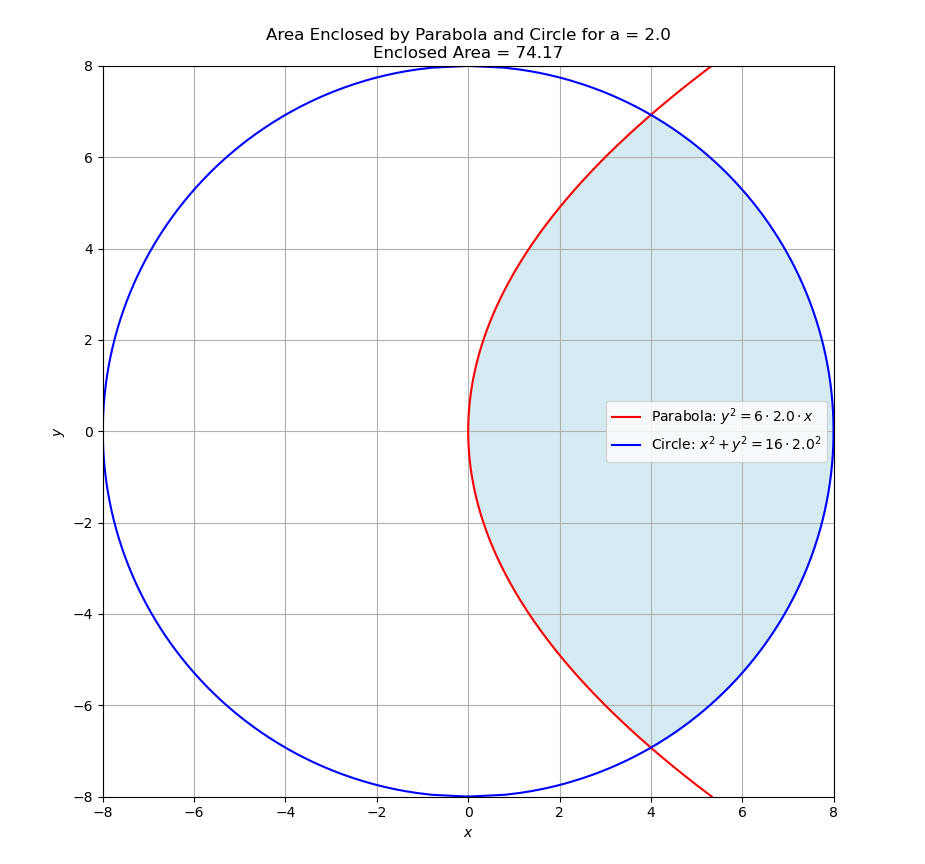
\includegraphics[width=0.7\textwidth]{figs/fig_2.png}
    \end{center}
    \vspace{0.5cm}
    \begin{itemize}
        \item The plot shows the intersection and enclosed area between the parabola \( y^2 = 6 \cdot 1.0 \cdot x \) (red) and the circle \( x^2 + y^2 = 16 \cdot 1.0^2 \) (blue).
        \item Calculated enclosed area: 18.54.
    \end{itemize}
\end{frame}
\begin{frame}[fragile]
    \frametitle{C Code to Generate Data for Python Script}

    \begin{lstlisting}
#include <stdio.h>
int main() {
    // Open the file to write the values of 'a'
    FILE *file = fopen("data.txt", "w");
    if (file == NULL) {
        printf("Error opening file!\n");
        return 1;
    }
    // Write the values of 'a' to the file (a = 1 and a = 2)
    fprintf(file, "1.0\n");
    fprintf(file, "2.0\n");
    // Close the file
    fclose(file);
    printf("Values of 'a' written to data.txt\n");

    return 0;
}
    \end{lstlisting}
\end{frame}
\begin{frame}[fragile]
    \frametitle{Loading Values of 'a' from Text File}

    \begin{lstlisting}
import numpy as np
import matplotlib.pyplot as plt
from scipy.integrate import quad
from scipy.optimize import fsolve

# Read the values of 'a' from the C-generated text file using numpy.loadtxt
data = np.loadtxt('data.txt')
a_values = data  # a_values will contain [1.0, 2.0]
    \end{lstlisting}

    This code loads the values of `a` from a text file, which contains values generated by the C code.
\end{frame}

\begin{frame}[fragile]
    \frametitle{Defining the Parabola and Circle Equations}

    \begin{lstlisting}
# Define the equation of the parabola: y^2 = 6ax, which implies x = y^2 / (6a)
def parabola(y, a):
    return y**2 / (6 * a)

# Define the equation of the circle: x^2 + y^2 = 16a^2, which implies x = sqrt(16a^2 - y^2)
def circle(y, a):
    return np.sqrt(16 * a**2 - y**2)
    \end{lstlisting}

    Here we define the equations for the parabola \( y^2 = 6ax \) and the circle \( x^2 + y^2 = 16a^2 \).
\end{frame}

\begin{frame}[fragile]
    \frametitle{Finding Intersection Points}

    \begin{lstlisting}
# Find the points of intersection between the parabola and the circle
def find_intersections(a):
    def intersection_eq(y):
        return circle(y, a) - parabola(y, a)
    
    # Solve for the y values of intersection
    y_int1 = fsolve(intersection_eq, -4 * a)[0]
    y_int2 = fsolve(intersection_eq, 4 * a)[0]

    return y_int1, y_int2
    \end{lstlisting}

    This function finds the points where the parabola and circle intersect by solving for \( y \).
\end{frame}

\begin{frame}[fragile]
    \frametitle{Computing the Enclosed Area}

    \begin{lstlisting}
# Compute the area between the curves using numerical integration
def area_between_curves(y, a):
    return circle(y, a) - parabola(y, a)

# Loop over each value of 'a' and compute the enclosed area
for a in a_values:
    y_int1, y_int2 = find_intersections(a)
    area, _ = quad(area_between_curves, y_int1, y_int2, args=(a,))
    print(f"Area enclosed between the parabola and the circle for a = {a}: {area}")
    \end{lstlisting}

    This code computes the area enclosed between the curves using numerical integration over each value of \( a \).
\end{frame}

\begin{frame}[fragile]
    \frametitle{Preparing to Plot the Curves}

    \begin{lstlisting}
    # Define y-values for plotting the parabola and the circle
    y_vals = np.linspace(-4 * a, 4 * a, 400)
    x_parabola = parabola(y_vals, a)
    x_circle_upper = circle(y_vals, a)
    x_circle_lower = -circle(y_vals, a)
    \end{lstlisting}

    This part of the code prepares \( y \)-values and corresponding \( x \)-values for plotting the parabola and circle.
\end{frame}

\begin{frame}[fragile]
    \frametitle{Plotting the Curves and Shading the Enclosed Area}

    \begin{lstlisting}
    # Plot the curves for this value of 'a'
    plt.figure()
    plt.plot(x_parabola, y_vals, label=r'Parabola: $y^2 = 6 \cdot %.1f \cdot x$' % a, color='red')
    plt.plot(x_circle_upper, y_vals, label=r'Circle: $x^2 + y^2 = 16 \cdot %.1f^2$' % a, color='blue')
    plt.plot(x_circle_lower, y_vals, color='blue')

    # Fill the area between the curves for each value of 'a'
    y_shaded = np.linspace(y_int1, y_int2, 400)
    plt.fill_betweenx(y_shaded, parabola(y_shaded, a), circle(y_shaded, a), 
                      where=(circle(y_shaded, a) >= parabola(y_shaded, a)),
                      color='lightblue', alpha=0.5)
    \end{lstlisting}

    This code plots the parabola, circle, and fills the area enclosed between them.
\end{frame}

\begin{frame}[fragile]
    \frametitle{Final Plot Settings and Display}

    \begin{lstlisting}
    # Labels and plot settings
    plt.xlabel('$x$')
    plt.ylabel('$y$')
    plt.title(f'Area Enclosed by Parabola and Circle for a = {a}\nEnclosed Area = {area:.2f}')
    plt.grid(True)
    plt.legend()

    # Set equal aspect ratio and axis limits for a clearer view
    plt.gca().set_aspect('equal', adjustable='box')
    plt.xlim(-8, 8)
    plt.ylim(-8, 8)
    \end{lstlisting}

    Here we add labels, title, legend, and set the plot limits for better visualization.
\end{frame}

\begin{frame}[fragile]
    \frametitle{Displaying the Plots}

    \begin{lstlisting}
# Show the plots for both values of 'a'
plt.show()
    \end{lstlisting}

    Finally, this command displays the plots for both values of \( a \) on separate figures.
\end{frame}
\begin{frame}{}
  \centering \Huge
  \emph{Thank You}
\end{frame}



\end{document}
